% Figure-only placement kit. Paths relative to manuscript/.
% Do not input wholesale: see FIGURE_INTEGRATION.md. Existing prose is untouched.

% Main Figure 1
\begin{figure*}[t]
\centering
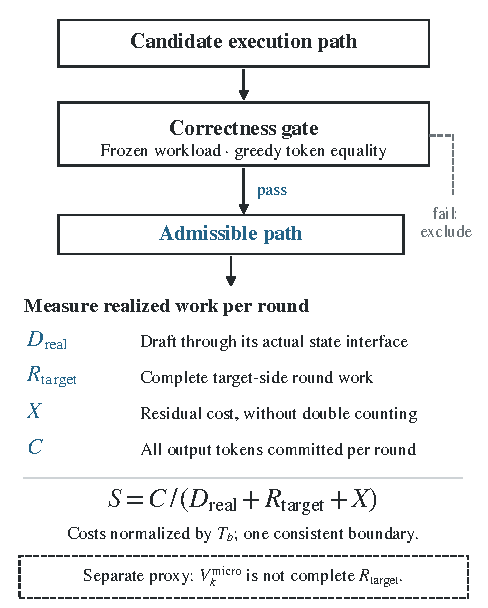
\includegraphics[width=\textwidth]{../figures/pdf/figure1.pdf}
\caption{\textbf{Favorable local signals, divergent realized outcomes}. Near-one-step target batching and favorable isolated drafting do not consistently translate into qualified end-to-end gains in the tested cases. The same tested M4 Metal stack exhibits a profitable HumanEval regime and a negative representative-24Q regime in separate frozen studies. RTX batched verification is physically cheap but fails correctness qualification. The 358H NPU has higher isolated median throughput at 8,192 tokens yet reaches only 0.352$\times$ realized speedup. Rows are heterogeneous case summaries, not a hardware ranking or common quantitative axis. M4 micro values describe the shared path in a separate micro study. Headline speedups cover post-prefill decode; Figures 2--4 give conditions, uncertainty and the two measured diagnoses.}
\label{fig:overview}
\end{figure*}

% Main Figure 2
\begin{figure*}[t]
\centering
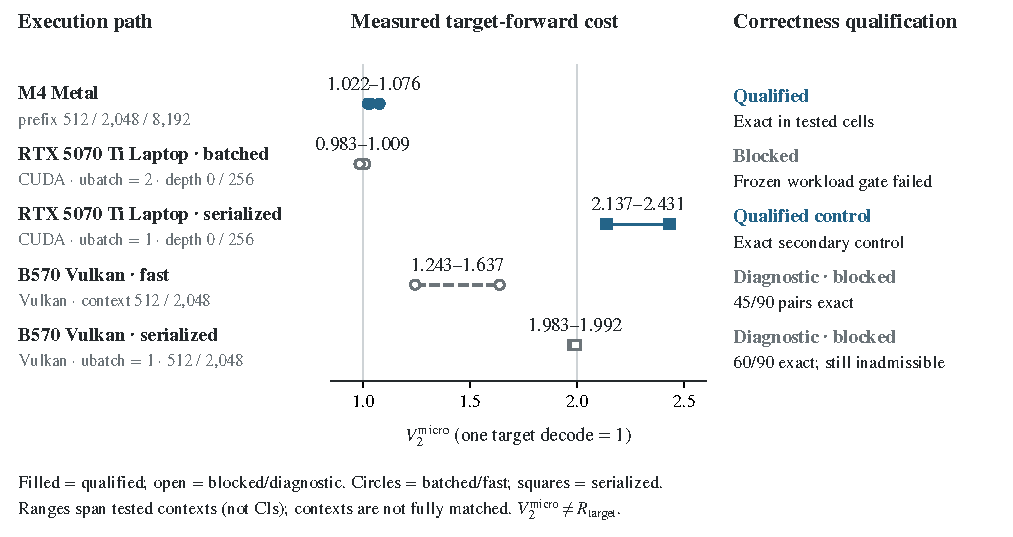
\includegraphics[width=\textwidth]{../figures/pdf/figure2.pdf}
\caption{\textbf{Correctness qualification changes which verification path is usable}. Each mark is one measured context cell; range segments span those cells, not confidence intervals. Filled markers indicate qualified tested paths; open markers indicate blocked or diagnostic paths. Serialization yields an exact secondary RTX control, but the B570 serialized diagnostic remains globally inadmissible despite improving observed exactness from 45/90 to 60/90 pairs. Contexts and runtime stacks are not fully matched. The target-forward proxy $V_2^{\mathrm{micro}}$ excludes complete realized target-side work $R_{\mathrm{target}}$ and is not an end-to-end speedup. Qualification is scoped to the frozen workload and execution path, not a device family.}
\label{fig:verification}
\end{figure*}

% Main Figure 3
\begin{figure}[t]
\centering
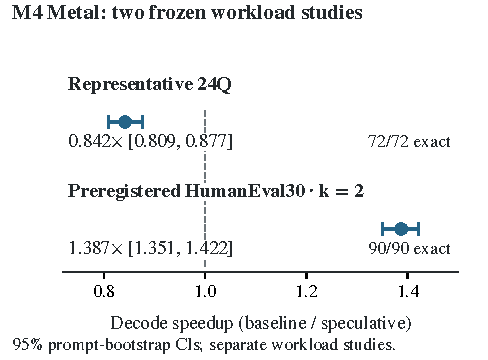
\includegraphics[width=\columnwidth]{../figures/pdf/figure3.pdf}
\caption{\textbf{Opposite profitability regimes on the same tested M4 stack}. Representative 24Q yields 0.842$\times$ [0.809, 0.877], while the separately preregistered HumanEval30 fixed-$k=2$ study yields 1.387$\times$ [1.351, 1.422]. Points are campaign prompt geometric means of paired decode speedups; intervals are campaign-specific 95\% prompt-bootstrap intervals. The dashed line marks parity. Both paths satisfy token equality (72/72 and 90/90 pairs), which is not functional HumanEval pass@$k$. These are separate studies, not a paired between-workload comparison; differing workloads and session conditions do not isolate workload-only causality.}
\label{fig:m4}
\end{figure}

% Main Figure 4
\begin{figure*}[t]
\centering
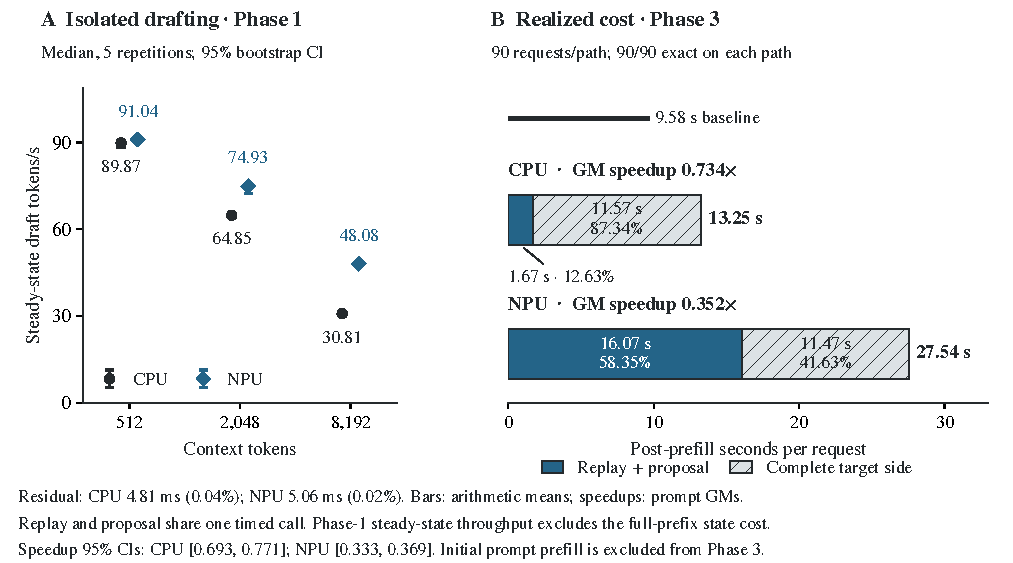
\includegraphics[width=\textwidth]{../figures/pdf/figure4.pdf}
\caption{\textbf{Isolated draft advantage does not survive the measured stateful integration}. (A) Phase-1 median steady-state draft throughput and 95\% repetition-bootstrap intervals, five repetitions per cell; the NPU median advantage grows across the tested contexts. (B) Phase-3 arithmetic mean post-prefill seconds per request over 90 observations per path, all exact. CPU and NPU totals are 13.25 s and 27.54 s against a 9.58 s mean baseline. The CPU path is target-side dominated (87.34\%); the NPU path spends 58.35\% in the measured replay-plus-proposal call. The 0.734$\times$ and 0.352$\times$ headlines use the separate prompt-GM estimator and are not ratios of the arithmetic mean bars. Replay and proposal cannot be separated within this timer. Initial prompt prefill is excluded. This diagnoses the tested runtime interface, not intrinsic NPU capability or a measured benefit from a state-persistent intervention. Together with Figure 2, it identifies two measured reasons local opportunity need not become realized gain; the M4 contrast remains a separate empirical observation.}
\label{fig:state}
\end{figure*}

% Appendix A1 only
\begin{figure*}[t]
\centering
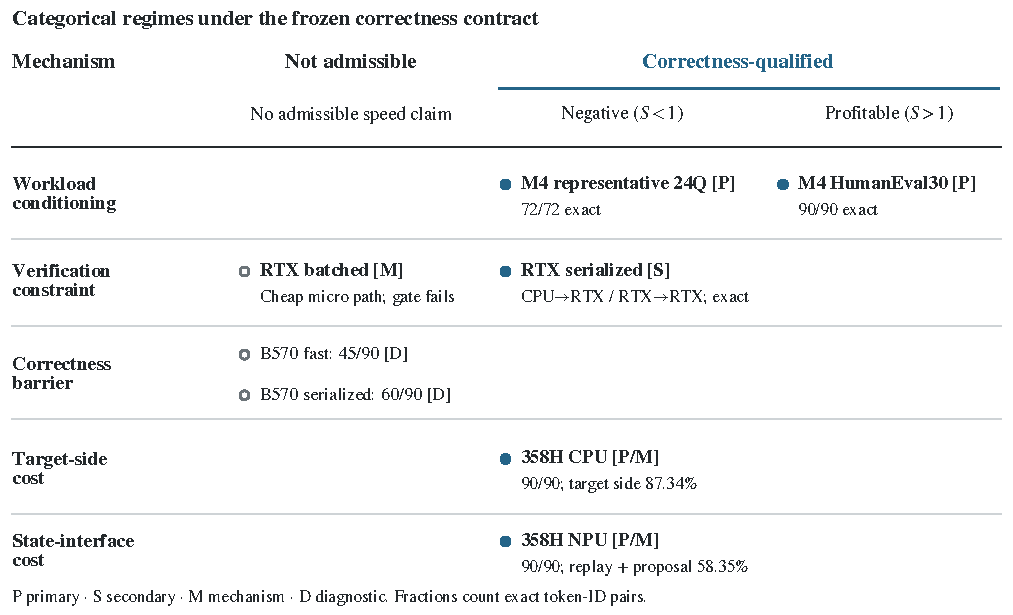
\includegraphics[width=\textwidth]{../figures/pdf/figure5.pdf}
\caption{\textbf{Evidence inventory across tested regimes}. Categorical columns distinguish globally blocked paths from exact negative and profitable regimes. Rows annotate observed constraints rather than define an exhaustive taxonomy. Both B570 paths remain diagnostic and globally inadmissible. RTX serialized controls are secondary evidence; 358H outcome and decomposition support primary and mechanism claims, respectively. Empty cells indicate no displayed case, not impossibility. No hardware ordering or continuous correctness metric is implied.}
\label{fig:regimes}
\end{figure*}
